\documentclass[12pt,letter]{article}
\usepackage{../downey_format}


\begin{document}
	
	% set the section number, along with figure and equation numbers
	\setcounter{section}{0}	
	\setcounter{figure}{0}   
	\renewcommand\thefigure{\thesection.\arabic{figure}}


\section{Text Overview}

\begin{itemize}
	\item Systems, 1\textsuperscript{st} order, 2\textsuperscript{nd} order, and higher order.
	\begin{itemize}
		\item Introduction to control systems		
		\item Differential equations
		\item General solution
		\item Free Response
		\item Stability 
		\item Laplace Transforms
	\end{itemize}
	\item Performance
	\begin{itemize}
		\item Time response
		\item Performance indicators
		\item System identification
	\end{itemize}
\item Control Systems
\begin{itemize}
	\item Feedback
	\item Stability
	\item Controllers 
\end{itemize}
\item Frequency Analysis
\begin{itemize}
	\item FRF
	\item Bode
	\item Nyquist
	\item Mangus 
\end{itemize}
\item Additional Topics
\begin{itemize}
	\item Combined Analysis
	\item CSD
	\item Single-input single-output (SISO)
	\item Tool
	\item State Space Models (introduction)
\end{itemize}

\end{itemize}



%		\begin{figure}[H]
%			\centering
%			\includegraphics[width=\linewidth]{../figures/simple_neural_network_vs_deep_learning.jpg}
%			\caption{simple neural network vs deep learning}
%			\label{fig:simple_neural_network_vs_deep_learning}
%		\end{figure}







\subsection{Basics of Control System}
A control system consisting of interconnected components is designed to achieve a desired purpose. To understand the purpose of a control system, it is useful to examine examples of control systems through the course of history. These early systems incorporated many of the same ideas of feedback that are in use today.

Modern control engineering practice includes the use of control design strategies for improving manufacturing processes, the efficiency of energy use, advanced automobile control, including rapid transit, among others. 



\noindent \textbf{System} - An interconnection of elements and devices for a desired purpose. \\


\noindent \textbf{Control System} - An interconnection of components forming a system configuration that will provide a desired response. \\

\noindent \textbf{Process} - The device, plant, or system under control. The input and output relationship represents the cause-and effect relationship of the process.


		\begin{figure}[H]
			\centering
			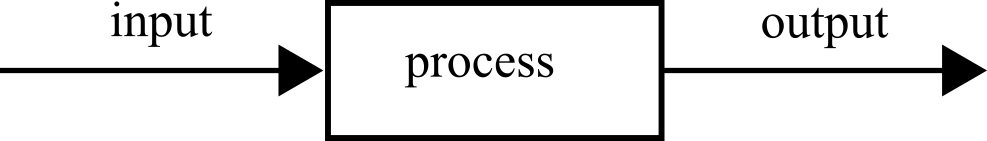
\includegraphics[]{../figures/control_system_input_output}
			\caption{Process to be controlled.}
			\label{fig:input_output_control_system}
		\end{figure}



\noindent \textbf{Open-Loop Control Systems} - utilize a controller or control actuator to obtain the desired response.


		\begin{figure}[H]
			\centering
			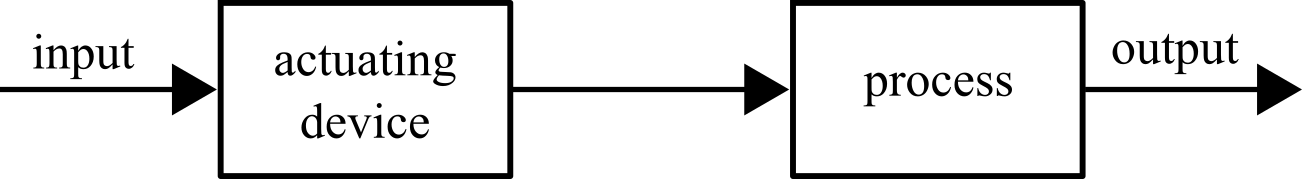
\includegraphics[]{../figures/control_system_open_loop}
			\caption{Open-loop control system (without feedback).}
			\label{fig:open_loop_control_system}
		\end{figure}

\noindent \textbf{Closed-Loop Control Systems} - utilizes feedback to compare the actual output to the desired output response.

		\begin{figure}[H]
			\centering
			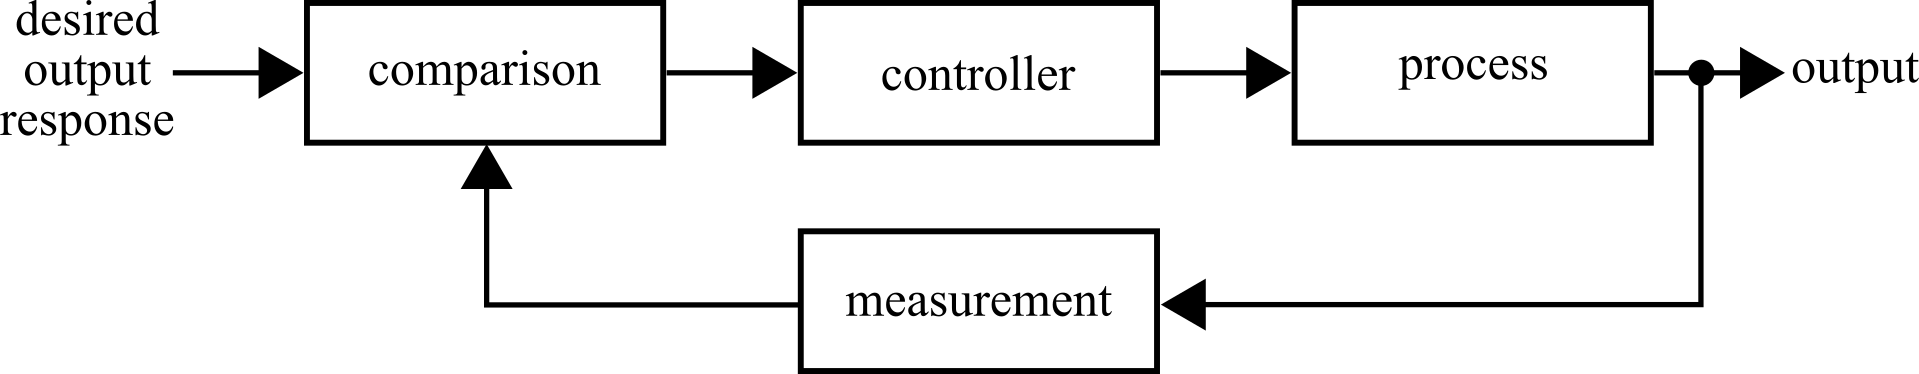
\includegraphics[width=4.5in]{../figures/control_system_closed_loop}
			\caption{Closed-loop control system (with feedback).}
			\label{fig:closed_loop_control_system}
		\end{figure}



\noindent \textbf{Multivariable Control System} - a control system with multiple desired response controlled by multiple output variables. 


		\begin{figure}[H]
			\centering
			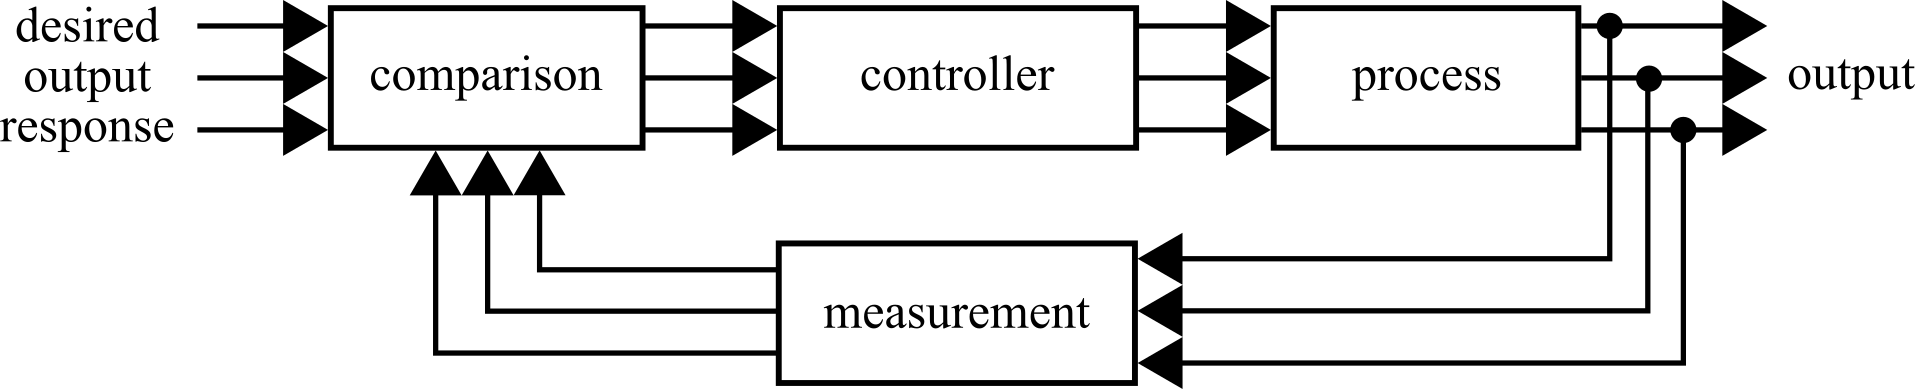
\includegraphics[width=4.5in]{../figures/control_system_closed_loop_multivariable}
			\caption{Multivariable control system with many inputs and many outputs to the system.}
			\label{fig:multivariable_control_system}
		\end{figure}


\noindent \textbf{Positive and negative feedback} - A positive feedback (also called Regenerative feedback) adds control outputs to the system in the same direction as the original perpetuation while a negative feedback (Degenerative feedback) provides a counteracting force to the original permutations.



\subsection{Videos of control systems}

\noindent \textbf{Ball and Plate PID control with 6 DOF Stewart platform}\\
\url{https://www.youtube.com/watch?v=j4OmVLc_oDw&t=95s&ab_channel=FullMotionDynamics}

\noindent \textbf{Ball and Plate PID control with 6 DOF Stewart platform}\\
\url{https://www.youtube.com/watch?v=meMWfva-Jio&ab_channel=StepanOzana}

\noindent \textbf{SpaceX first landing}\\
\url{https://www.youtube.com/watch?v=1sJlFzUQVmY&ab_channel=BloombergQuicktake}


\subsection{History}

\begin{itemize}
\item Greece (BC) - Float regulator mechanism.
\item Holland (16th Century) - Temperature regulator.
\item 18th Century James Watt's centrifugal governor for the speed control of a steam engine. 
\item 1920s Minorsky worked on automatic controllers for steering ships.
\item 1930s Nyquist developed a method for analyzing the stability of controlled systems.
\item 1940s Frequency response methods made it possible to design linear closed-loop control systems.
\item 1950s Root-locus method due to Evans was fully developed.
\item 1960s State space methods, optimal control, adaptive control.
\item 1980s Learning controls are begun to investigated and developed.
\item Present and on-going research fields. Recent application of modern control theory includes such non-engineering systems such as biological, biomedical, economic and socio-economic systems
\end{itemize}

\subsection{Examples of control systems}

Controllers in the form of centrifugal governors for steam engines set off the industrial revolution by allowing steam engines to produce reliable and controllable power. Figure~\ref{fig:steam_engines} shows centrifugal governor on steam engines. 

		\begin{figure}[H]
			\centering
			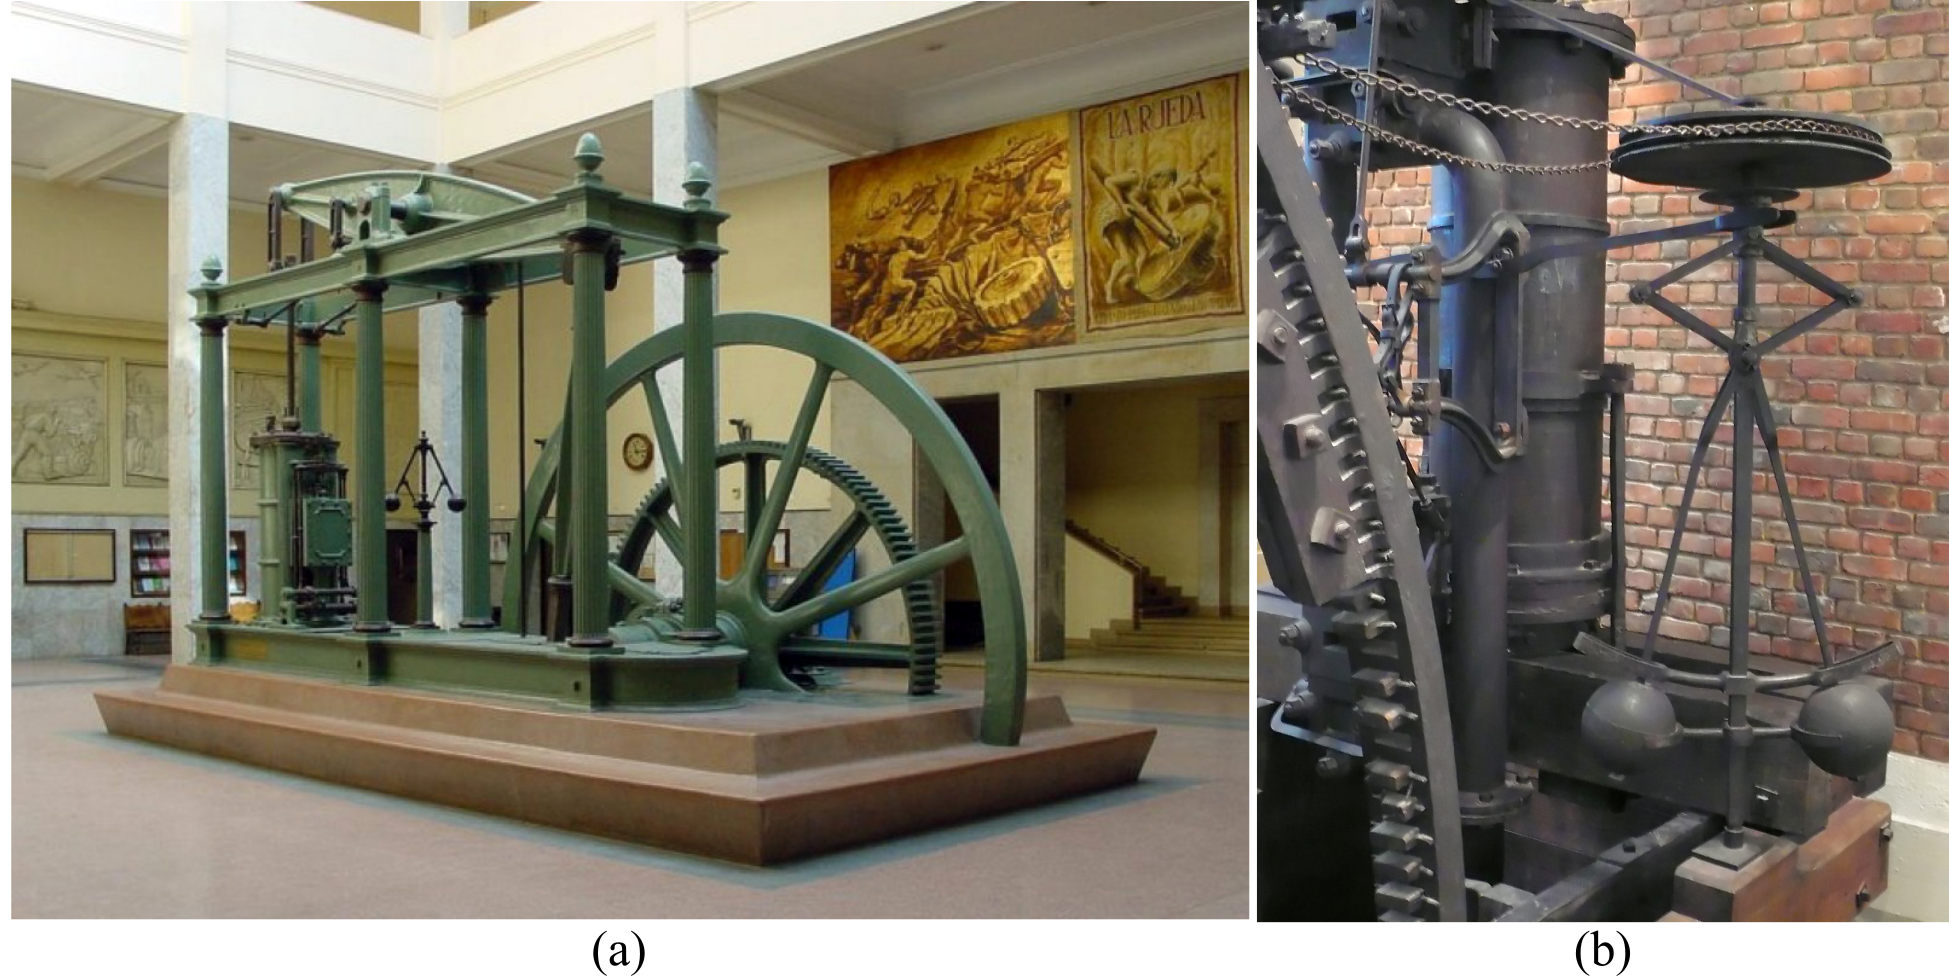
\includegraphics[]{../figures/steam_engines}
			\caption{Centrifugal governors on a: (a) Boulton \& Watt steam engine from 1788 \protect\footnotemark[1], and; (b) D. Napier \& Son from 1832 double-acting steam engine \protect\footnotemark[2].}
			\label{fig:steam_engines}
		\end{figure}
	\footnotetext[1]{Dr. Mirko Junge, CC BY 3.0 $<$https://creativecommons.org/licenses/by/3.0$>$, via Wikimedia Commons.}
	\footnotetext[2]{Nicol�s P�rez, CC BY-SA 3.0 $<$http://creativecommons.org/licenses/by-sa/3.0/$>$, via Wikimedia Commons.}

\pagebreak
		Arguably, the Russian American engineer Nicolas Minorsky was the first to develop the theoretical analysis for the three-term control we now call PID. This was done in 1922 while he was researching and designing automatic ship steering for the US Navy. He based his work on watching how a ship's helmsman responds to wave loading on a ship, with a delayed input to the helm that not only considered the current ship course, but also past error and the desired rate of change for the ship. For a helmsman, the goal is stability, not absolute control, which simplifies how one thinks about the challenge of control.

\begin{figure}[H]
	\centering
	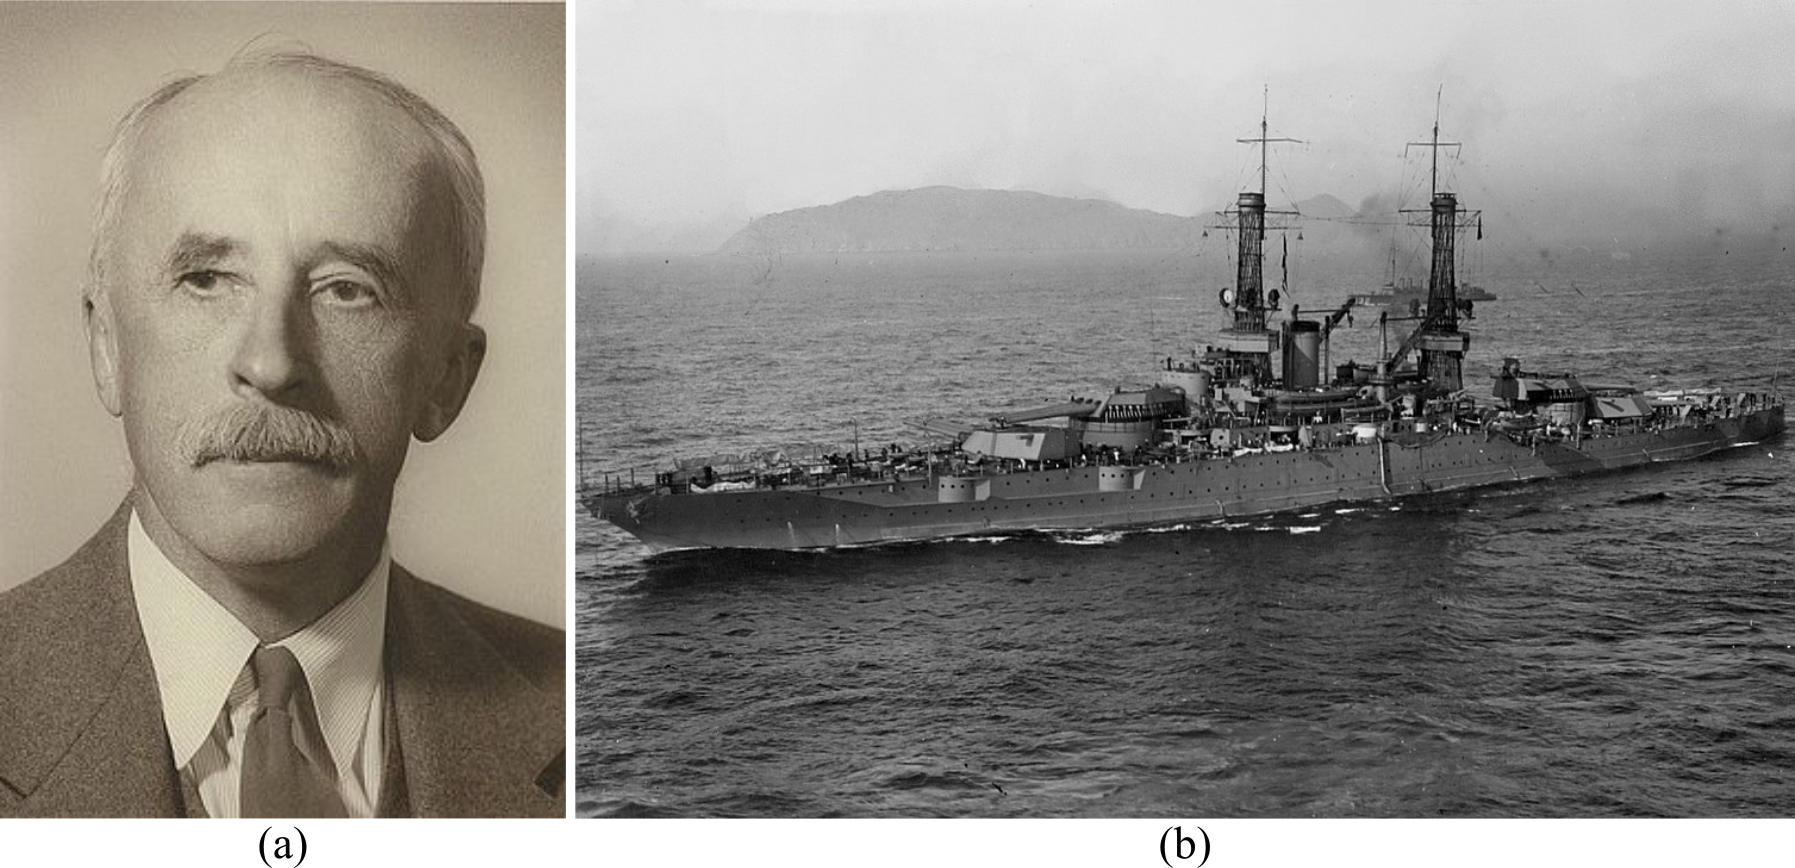
\includegraphics[]{../figures/PID_Nicolas_Minorsky_and_USS_New_Mexico.png}
	\caption{Historical prospective of PID control showing: (a) Portrait of Nicolas Minorsky \protect\footnotemark[1] and (b) the battleship USS New Mexico (BB-40) of the United States Navy which was the first to implement PID control in its steering \protect\footnotemark[2]. }
	\label{fig:fragility_curve}
\end{figure}
	\footnotetext[1]{Peter Minorsky, grandson of Nicolas Minorsky, CC BY-SA 1.0 $<$https://creativecommons.org/licenses/by-sa/1.0$>$, via Wikimedia Commons} 
\footnotetext[2]{U.S. Navy, Public domain, via Wikimedia Commons} 



%\includepdf[pages=-,pagecommand={},width=0.9\textwidth]{PDF_notes/basics_of_control_system.pdf}
%
% \cite{Halevy2009UnreasonableEffectivenessData}
%
%
%
%	\pagebreak
%	\renewcommand{\thepage}{}
%	\renewcommand\refname{References Cited}
%	\pagestyle{plain}
%	\bibliographystyle{Downey_NSF}
%	\bibliography{Chapter_1_Basic_Concepts}


















\end{document}

